\section{Theorie}

\subsection{Beugung}

\subsubsection{Allgemeine Definition}

Als Beugung bezeichnet man das Ph\"anomen, dass Licht, welches durch begrenzende \"Offnungen oder an begrenzenden Kanten vorbeil\"auft, von seiner urspr\"unglichen Richtung abgelenkt wird. Hinter dem Hindernis \"uberlagern sich die Teilwellen gem\"a\ss \ dem Huygenschen Prinzip, welches besagt, dass jeder Punkt einer Wellenfront eine neue Welle induziert. Diese \"uberlagern sich dann und die daraus resultierenden Interferenzerscheinungen werden als Beugung bezeichnet.

\subsubsection{Das Kirchhoff'sche Beugungsintegral}

\begin{figure}[H]
	\centering 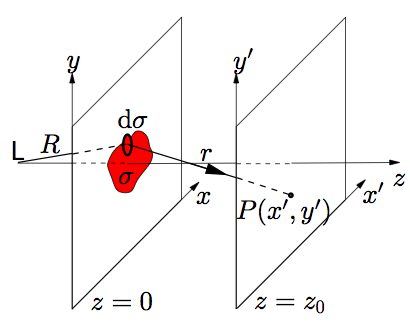
\includegraphics[width=0.5\textwidth]{Bilder/Beugungsintegral.jpg}
	\caption{Zum Kirchhoffschen Beugungsintegral}
\end{figure}

Licht mit der Amplitude $E_\sigma$, welches auf die Blenden\"offnung $\sigma$ f\"allt, hat im Punkt $P$ auf dem Schirm hinter der \"Offnung die Amplitude: $$dE_P = C\frac{E_\sigma \cdot d\sigma}{r}e^{-ikr}$$
($C$ ist hier ein Proportionalit\"atsfaktor)\\
Betrachtet man die Beitr\"age aller $d\sigma$, so erh\"alt man das Fresnel-Kirchhoffsche Beugungsintegral:
$$E_P=\iint C\cdot E_\sigma \cdot \frac{e^{-ikr}}{r}dxdy$$

Dieses Integral kann man nun mit der Fraunhofer-N\"aherung als Fourierintegral umwandeln. Die Fraunhofer-N\"aherung ist eine Fernfeldn\"aherung; die Spaltgr\"o\ss e wird als klein angenommen und die Lichtquelle als sehr weit entfernt. Mit diesen Vereinfachungen wird das Integral zu:

$$ E(x',y') = A(x',y',z_0)\cdot \iint E_{ein}(x,y)\cdot g(x,y)\cdot \exp(-i2\pi(x'x+y'y)/(\lambda z_0)) dxdy $$

und es gilt der Zusammenhang:

$$ E(x',y',z_0) = F(u,v) \cdot A(x',y',z_0)$$

wobei \begin{itemize}
\item $F(u,v)$ das Fourierintegral der Funktion $f(x,y) = g(x,y)\cdot E_{ein}(x,y)$
\item $g(x,y)$ die Aperturfunktion der \"Offnung
\item $A(x',y',z_0)=\frac{e^{-ikz_0}}{i\lambda z_0}\cdot e^{i\pi (x'^2 + y'2) / \lambda z_0}$ und $|A|^2 =1$
\end{itemize}

Somit folgt f\"ur die Intensit\"at:

$$I \sim |E|^2 = \left| \iint g(x,y)\cdot e^{ikr} dxdy \right|^2 $$

Im Allgemeinen kann man auch aus der Intensit\"atsverteilung die Aperturfunktion herleiten, indem man eine inverse Fouriertransformation macht. Man kann die Transformation durch eine Fourierreihe n\"ahern, die die Wurzeln der Peak-Amplituden als Argumente hat:

$$g(x) = \sum_{n=0}^m \pm \sqrt{I_n} \cos\left(\frac{2\pi n}{K}x\right)$$


\subsubsection{Beugung an Amplitudengittern}

\begin{enumerate}
 
\item Beugung am Einzelspalt


\begin{minipage}{0.6\textwidth}
Die Aperturfunktion am Einzelspalt (unter Vernachl\"assigung der Begrenzung in y-Richtung) lautet:
$$ g(x) = \begin{cases} 
	1 & \text{, falls} -\frac{b}{2}<x<\frac{b}{2}\\
	0 & \text{, sonst}
     \end{cases}$$
Man erh\"alt durch Ausrechnen des Beugungsintegrals folgende Abh\"angigkeit f\"ur die Intensit\"at:
$$ I \sim \left(\frac{\sin(\beta)}{\beta}\right)^2 $$
\end{minipage}
\begin{minipage}{0.4\textwidth}
	\begin{center}
		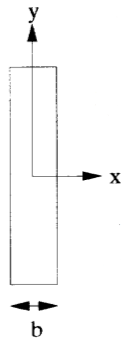
\includegraphics[width=0.35\textwidth]{Bilder/Einzelspalt.jpg}
	\end{center}
\end{minipage}

Hier ist $\beta = \frac{kb}{2}\sin(\theta)$, $k = \frac{2\pi}{\lambda}$ und $\theta$ der Einfallswinkel auf dem Schirm vom Ursprung des Spaltes aus.

\item Beugung am Gitter

\begin{minipage}{0.6\textwidth}
Ein Gitter besteht aus N Einzelspalten nebeneinander angeordnet. Alle Spalten haben idealerweise die Breite $b$ und die Distanz $K$ voneinander in $x$-Richtung. $K$ wird als Gitterkonstante bezeichnet. Die Aperturfunktion f\"ur das Gitter lautet somit:

$$ g(x) = \begin{cases} 
	1 & \text{, falls \ \ } N\cdot K\leq x \leq N\cdot K+b \text{\ mit \ } N \in \mathbb{N}\\
	0 & \text{, sonst}
     \end{cases}$$
     
\end{minipage}
\begin{minipage}{0.4\textwidth}
	\begin{center}
		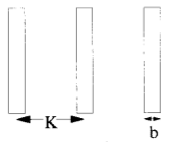
\includegraphics[width=0.7\textwidth]{Bilder/Gitter.jpg}
	\end{center}
\end{minipage}

F\"ur die Intensit\"atsverteilung folgt hier:

$$I \sim \left(\frac{\sin(\beta)}{\beta}\right)^2\cdot \left(\frac{\sin(N\gamma)}{N\cdot \sin(N\gamma)}\right)^2 $$

mit $\gamma = \frac{1}{2}\cdot k\cdot K\cdot \sin(\theta)$ und $\beta$ wie oben.

Der linke Faktor beschreibt die Einh\"ullende der Intensit\"atsverteilung am Schirm, und der rechte Faktor beschreibt die Intensit\"atspeaks. Wenn der Gangunterschied von zwei Elementarwellen ein Vielfaches der Wellenl\"ange des Lichts ist, so erh\"alt man am Schirm ein Intensit\"atsmaximum. Man erh\"alt die Beziehung

$$ m \cdot \lambda = K\cdot \sin(\theta) \text{,} $$

die die Position der Maxima beschreibt.

\item Sinusgitter

Die Aperturfunktion eines Sinusgitters lautet:

$$g(x) = \sqrt{I_0} + \sqrt{I_1} \cdot \cos \left( \frac{2\pi}{K}x \right) $$

Man hat also nur Maxima 0. und 1. Ordnung in der Intensit\"atsverteilung:

\begin{figure}[H]
	\centering 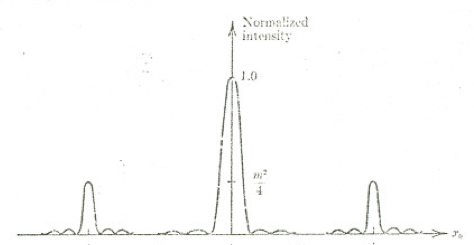
\includegraphics[width=0.7\textwidth]{Bilder/Sinusverteilung.jpg}
	\caption{Intesit\"atsverteilung vom Sinusgitter}
\end{figure}
\end{enumerate}

\subsubsection{Aufl\"osungsverm\"ogen}

Das Aufl\"osungsverm\"ogen ist definiert durch $$a=\frac{\lambda}{\Delta \lambda}$$

wobei $\lambda +\Delta \lambda$ die Wellenl\"ange ist, die sich bei der Beugung noch von $\lambda$ unterscheiden l\"asst. F\"ur ein Gitter mit $N$ durchleuchteten Spalten und $m$ sichtbaren Maxima ergibt sich die Aufl\"osung $$a=N\cdot m$$




































